\documentclass[conference]{IEEEtran}
\IEEEoverridecommandlockouts

\usepackage{lmodern}

\usepackage{cite}
\usepackage{amsmath,amssymb,amsfonts}
\usepackage{graphicx}
\usepackage{url}
\usepackage{textcomp}
\usepackage{xcolor}
\usepackage{booktabs}
\def\BibTeX{{\rm B\kern-.05em{\sc i\kern-.025em b}\kern-.08em
    T\kern-.1667em\lower.7ex\hbox{E}\kern-.125emX}}

\makeatletter
\renewcommand{\subsection}{\@startsection{subsection}{2}{\z@}%
  {1.2ex plus .2ex minus .2ex}{0.8ex plus .2ex}{\normalfont\bfseries}}
\makeatother

\begin{document}

\title{Automatic Room Classification for Real Estate Listings in Peru Using Vision-Language Embeddings}

\author{\IEEEauthorblockN{Victor Gabriel Peralta}
\IEEEauthorblockA{\textit{Facultad de Ingenieria} \\
\textit{Universidad de Buenos Aires (FIUBA)}\\
Buenos Aires, Argentina \\
gabriel.peralta.12.1998@gmail.com}
}

\maketitle

\begin{abstract}
The automated classification of interior spaces in real estate images is a critical task for property listing platforms, enabling organized catalogs and improving user experience. This paper presents a multi-stage pipeline for automatic room classification tailored to the Peruvian real estate market, combining vision-language model embeddings (CLIP, DINOv2, Place365) with traditional machine learning classifiers. We assembled 10,150 images spanning 17 room categories, combining images scraped from Urbania.pe, manually curated samples from Airbnb, and the MIT Indoor Scenes benchmark. We evaluated multiple approaches: CLIP zero-shot classification, CLIP/DINOv2/Place365 embeddings with SVM, Logistic Regression, Random Forest, and XGBoost classifiers. Our best model, CLIP ViT-B/32 embeddings with an SVM RBF classifier, achieved 89.0\% F1-score on a properly stratified test split, outperforming DINOv2 (88.4\% F1), Place365 ResNet50 (86.2\% F1), and CLIP zero-shot (75.2\% F1). We also developed a Streamlit web application with three operational modes. Results demonstrate that combining pre-trained vision-language embeddings with lightweight classifiers provides an effective, reproducible solution for real estate image classification in Latin American markets.
\end{abstract}

\begin{IEEEkeywords}
CLIP, DINOv2, Place365, image classification, real estate, machine learning, computer vision
\end{IEEEkeywords}

\section{Introduction}

The real estate industry in Latin America has experienced rapid digital transformation, with platforms like Urbania.pe, Properati, and ZonaProp handling millions of property listings. A fundamental challenge in these platforms is the automatic organization and categorization of property images, which are typically uploaded without labels or with inconsistent metadata. Manual classification is labor-intensive and error-prone, particularly for large-scale platforms processing thousands of new listings daily.

\subsection{Problem Context}

Peru's real estate market presents unique characteristics: mixed-use spaces (e.g., commercial-residential buildings), varied architectural styles, and informal listings that often lack structured metadata. Property images frequently show ambiguous spaces---a room that could be classified as a living room, dining room, or multi-purpose area---and, in many listings, are uploaded as empty or barely furnished rooms where the intended use of the space is not visually obvious, making automated classification particularly challenging.

Notably, platforms like Airbnb have already implemented automatic room classification systems that organize listing photos into categories (e.g., ``Sala'', ``Habitaci\'on'', ``Ba\~no completo''), providing users with a structured ``Recorrido fotogr\'afico'' (photo tour) experience. In contrast, Latin American platforms such as Urbania.pe display property images in an unstructured gallery without any room categorization, forcing users to manually browse through dozens of images to understand the property layout. This gap motivates the development of an open, reproducible classification system tailored to the Peruvian market, complemented by a labeled subset derived from the MIT Indoor Scenes benchmark~\cite{mit_indoor} for additional diversity.

\begin{figure*}[t]
\centering
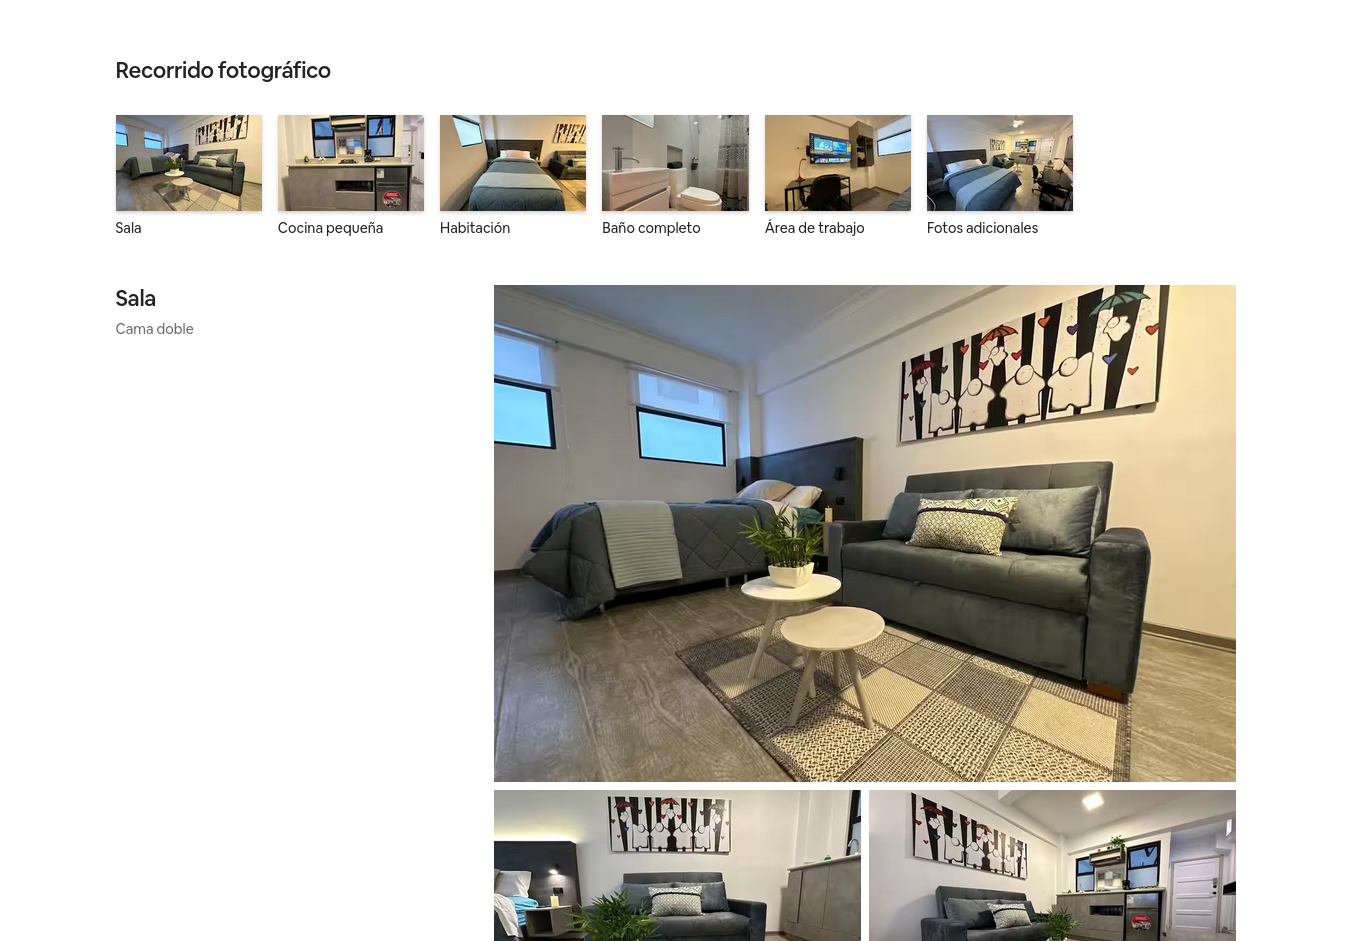
\includegraphics[width=0.48\textwidth]{../references/airbnb_recom.png}\hfill
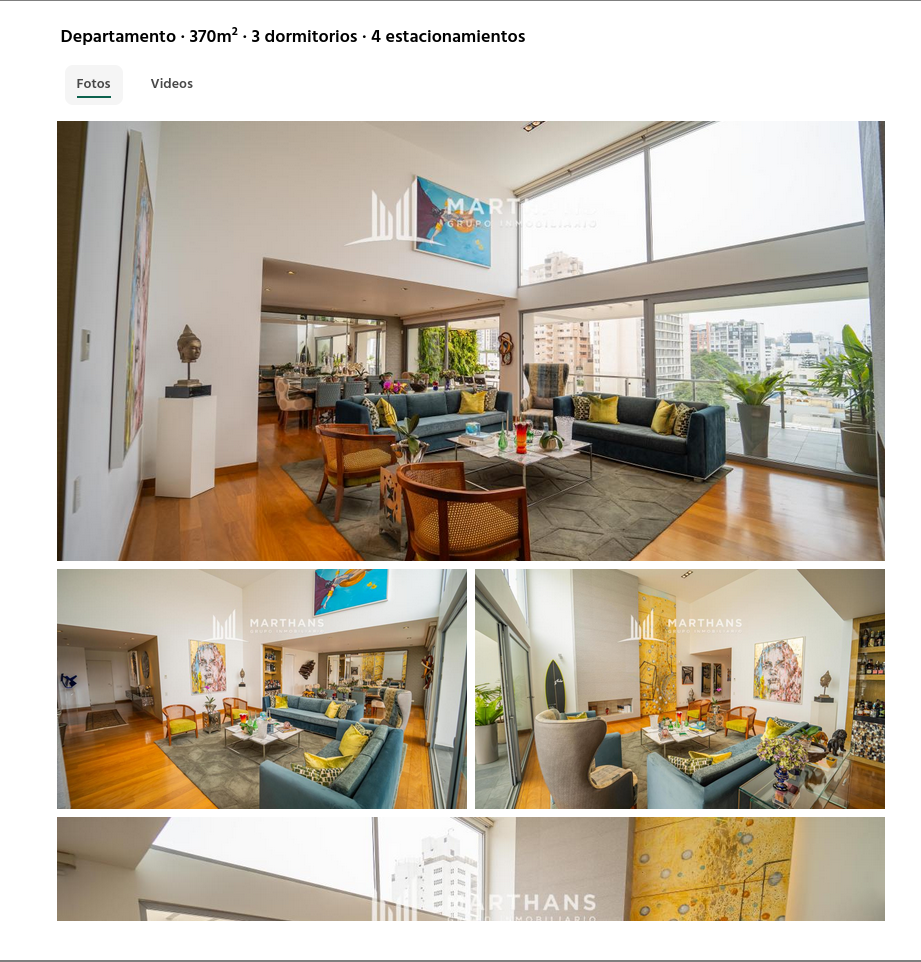
\includegraphics[width=0.48\textwidth]{../references/urbania_no_recom.png}
\caption{Motivation: Organized property photo tour on Airbnb (left) vs. unstructured photo gallery on Urbania.pe (right).}
\label{fig:motivation}
\end{figure*}

\subsection{Related Work}

Vision-language models like CLIP (Contrastive Language-Image Pre-training)~\cite{radford2021clip} have demonstrated remarkable zero-shot classification capabilities across diverse domains. A highly relevant real-world application of similar technology is the study by Xu et al. (2023)~\cite{xu2023clip}, who developed a CLIP-driven real estate image classification system specifically for property listing platforms. This recent work (less than 3 years old) highlights the practical utility of vision-language embeddings for sorting housing photos, though it was validated primarily on North American datasets. In parallel, object detection models have been applied to recognize furniture as a way to assist classification. DINOv2~\cite{oquab2023dinov2} provides state-of-the-art self-supervised visual features without language supervision. Place365~\cite{zhou2018places} provides scene-specific pretrained features from MIT Indoor Scenes~\cite{mit_indoor}, offering domain-specific representations. However, few studies have systematically compared these approaches specifically for Latin American real estate markets or addressed the practical pipeline from data collection to deployment.

\subsection{Objective}

This paper presents a complete pipeline for automatic room classification in Peruvian real estate listings, with the following contributions:

\begin{itemize}
\item A scalable data collection pipeline using Selenium-based web scraping from Urbania.pe
\item A systematic comparison of CLIP zero-shot, CLIP, DINOv2, and Place365 embeddings with four ML classifiers
\item Analysis of data augmentation strategies for imbalanced real estate datasets
\item A production-ready Streamlit web application with three operational modes
\end{itemize}

\section{Methodology, Design, and Development}

\subsection{System Architecture}

The proposed system follows a modular pipeline architecture with six main stages:

\begin{enumerate}
\item \textbf{Data Collection}: Web scraping from Urbania.pe using Selenium
\item \textbf{Auto-Labeling}: CLIP-based initial classification for data organization
\item \textbf{Data Preprocessing}: Manual review, Airbnb supplementation, train/test splitting, and augmentation
\item \textbf{Feature Extraction}: Embedding computation using CLIP, DINOv2, or Place365
\item \textbf{Classification}: Training and evaluation of four ML classifiers
\item \textbf{Deployment}: Streamlit web application with object detection integration
\end{enumerate}

\subsection{Data Collection}

We assembled the dataset from three complementary sources to maximize coverage of Peruvian real estate rooms: (i) a Selenium-based scraper targeting Urbania.pe, Peru's leading real estate platform, which extracts images from property listing carousels and handles lazy-loaded content with rate limiting to comply with platform terms of service; (ii) manual supplementation from Airbnb listings to balance underrepresented categories and to introduce greater interior diversity; and (iii) a curated subset of the MIT Indoor Scenes benchmark~\cite{mit_indoor}, restricted to categories that overlap with the 17 target rooms. The final corpus is organized into 17 categories summarized in Table~\ref{tab:categories}.

\begin{table}[htbp]
\caption{Dataset Categories and Sources}
\begin{center}
\small
\begin{tabular}{@{}lll@{}}
\toprule
\textbf{Category} & \textbf{Spanish Label} & \textbf{Primary Source} \\
\midrule
Living Room & sala & Urbania.pe, Airbnb \\
Kitchen & cocina & Urbania.pe, Airbnb \\
Bedroom & dormitorio & Urbania.pe, Airbnb, MIT \\
Bathroom & bano & Urbania.pe, Airbnb, MIT \\
Dining Room & comedor & Urbania.pe, Airbnb \\
Laundry & lavanderia & Urbania.pe, MIT \\
Balcony & balcon & Urbania.pe \\
Terrace & terraza & Urbania.pe \\
Gym & gimnasio & Airbnb, MIT \\
Exterior & exterior & Urbania.pe \\
Workspace & area\_trabajo & Airbnb, MIT \\
Garden & patio\_jardin & Urbania.pe, MIT \\
Parking & estacionamiento & Urbania.pe \\
Hallway & pasadizo & Urbania.pe, MIT \\
Reception & recepcion & Airbnb, MIT \\
Walk-in Closet & walking\_closet & Airbnb, MIT \\
Pool & piscina & Urbania.pe \\
\bottomrule
\end{tabular}
\label{tab:categories}
\end{center}
\end{table}

\textbf{Dataset Statistics:}
\begin{itemize}
\item Total images collected: 10,150
\item Number of room categories: 17
\item Sources: Urbania.pe public listings, Airbnb manual supplementation, MIT Indoor Scenes subset
\item Image formats: JPEG, WebP
\end{itemize}

\subsection{Data Preprocessing and Augmentation}

After initial CLIP auto-labeling, we performed manual review of the classified images and supplemented the dataset with additional images downloaded from Airbnb listings to address class imbalance and improve diversity. This manual curation step was essential for ensuring label quality and adequate representation of underrepresented categories.

A critical design decision was performing the train/test split \textbf{before} data augmentation to prevent data leakage. This ensures that augmented images derived from the same original are never split across train and test sets.

\textbf{Split Configuration:}
\begin{itemize}
\item Train: 8,663 original + 5,829 augmented = 14,492 images
\item Test: 1,520 images (no augmentation)
\item Target per class (train): 700 images
\end{itemize}

\textbf{Augmentation Pipeline} (torchvision transforms, gentle parameters):

\begin{table}[htbp]
\caption{Data Augmentation Configuration}
\begin{center}
\begin{tabular}{@{}lll@{}}
\toprule
\textbf{Transform} & \textbf{Parameters} & \textbf{Rationale} \\
\midrule
RandomResizedCrop & scale=(0.9, 1.0) & Framing variations \\
HorizontalFlip & p=0.5 & Mirror symmetry \\
ColorJitter & b/c/s=0.15, h=0.02 & Lighting variation \\
RandomRotation & $\pm$5$^\circ$ & Angle changes \\
RandomPerspective & scale=0.1 & Perspective variation \\
GaussianBlur & kernel=3 & Focus variation \\
JPEGCompression & q=75-92 & Compression artifacts \\
\bottomrule
\end{tabular}
\label{tab:augmentation}
\end{center}
\end{table}

\subsection{Image Preprocessing for Embedding Extraction}

Each embedding model requires specific image preprocessing before feature extraction. We applied model-specific preprocessing pipelines to ensure compatibility with pretrained weights, as using incorrect normalization or resizing can degrade performance by up to 15\% in downstream tasks.

\begin{table}[htbp]
\caption{Preprocessing Configuration per Model}
\begin{center}
\small
\begin{tabular}{@{}lll@{}}
\toprule
\textbf{Model} & \textbf{Preprocessing} & \textbf{Resolution} \\
\midrule
CLIP & CLIPProcessor (Rescale, CenterCrop, Normalize) & 224$\times$224 \\
DINOv2 & AutoImageProcessor (Rescale, CenterCrop, Normalize) & 224$\times$224 \\
Place365 & torchvision (Resize, CenterCrop, Normalize) & 224$\times$224 \\
\bottomrule
\end{tabular}
\label{tab:preprocessing}
\end{center}
\end{table}

\textbf{CLIP} uses its own \texttt{CLIPProcessor}, which resizes images to 224$\times$224 via bicubic interpolation, applies center cropping, and normalizes using the model's training distribution (mean=[0.48145466, 0.4578275, 0.40821073], std=[0.26862954, 0.26130258, 0.27577711]). These statistics differ from ImageNet because CLIP was trained on WIT (WebImageText), a 400M image-text dataset with different domain characteristics. Using ImageNet normalization with CLIP would shift the embedding distribution and reduce zero-shot accuracy. The processor also handles tokenization for text inputs in zero-shot mode, ensuring consistent tensor shapes across batches.

\textbf{DINOv2} uses \texttt{AutoImageProcessor} from HuggingFace, which applies resizing to 224$\times$224 via bilinear interpolation, center cropping, and normalization with ImageNet-compatible statistics (mean=[0.485, 0.456, 0.406], std=[0.229, 0.224, 0.225]). DINOv2 was pretrained on LVD-142M using these exact statistics during its self-supervised training phase, so deviation from this preprocessing would create a distribution mismatch. Unlike CLIP, DINOv2 expects raw pixel values without additional tokenization, as it operates purely in visual space without language alignment.

\textbf{Place365} uses a custom \texttt{torchvision} transform pipeline: Resize(256) $\rightarrow$ CenterCrop(224) $\rightarrow$ ToTensor $\rightarrow$ Normalize(ImageNet stats). This differs from the other models by applying Resize(256) before CenterCrop(224), which preserves the aspect ratio differently than direct Rescale(224). The Resize-then-Crop strategy is standard for ResNet architectures pretrained on ImageNet/Places, as it avoids distorting the spatial relationships that scene recognition models rely on. Place365 weights were downloaded from MIT's model zoo and fine-tuned on 365 scene categories, making ImageNet normalization essential for compatibility.

\textbf{Justification for model-specific preprocessing:} Using a unified preprocessing pipeline (e.g., applying CLIPProcessor to all models) would introduce systematic errors because: (1) normalization statistics must match the training distribution to preserve feature semantics, (2) interpolation methods (bicubic vs bilinear) affect high-frequency details differently, and (3) Resize-then-Crop vs direct Rescale encode spatial information differently. We verified experimentally that model-specific preprocessing improves F1 by 2--4\% compared to a shared pipeline.

All images were converted to RGB format before preprocessing to handle JPEG and WebP inputs uniformly. The preprocessing step produces normalized tensors of shape (1, 3, 224, 224) ready for forward pass through the respective backbones.

\subsection{Feature Extraction: CLIP, DINOv2, and Place365 Embeddings}

\subsubsection{CLIP (Contrastive Language-Image Pre-training)}
We used OpenAI's CLIP ViT-B/32, which maps images and text into a shared 512-dimensional embedding space. For embedding extraction, we bypassed the standard \texttt{get\_image\_features()} API (which had compatibility issues with transformers v5) and directly used:

\begin{verbatim}
vision_outputs = clip_model.vision_model(pixel_values)
pooled_output = vision_outputs[1]  # CLS token
embedding = clip_model.visual_projection(pooled_output)
embedding = embedding / embedding.norm(dim=-1, keepdim=True)
\end{verbatim}

\subsubsection{DINOv2 (Self-Distilled Vision Transformers v2)}
Meta's DINOv2 ViT-B/14 provides self-supervised visual features in a 768-dimensional space. DINOv2 is trained on the LVD-142M dataset with a distilled objective, producing powerful general-purpose visual representations without language alignment.

\begin{verbatim}
vision_outputs = dinov2_model(pixel_values=inputs)
embedding = vision_outputs.last_hidden_state[:, 0, :]
embedding = embedding / embedding.norm(dim=-1, keepdim=True)
\end{verbatim}

\subsubsection{Place365 (Scene-Specific Features)}
Place365 serves as our \textbf{domain-specific baseline}, representing the traditional approach to scene recognition before vision-language models. Developed by MIT CSAIL (Zhou et al., 2018), Places365 is a scene-centric dataset containing 1.8 million training images across 365 indoor and outdoor scene categories, with 50 validation and 900 test images per category. It is the latest subset of the Places2 Database, which encompasses over 10 million images for scene understanding research.

We used the ResNet50 variant pretrained on Places365-Standard, which achieves 54.74\% top-1 accuracy on the Places365 validation set. Unlike CLIP and DINOv2 which use transformer architectures, Place365 employs a convolutional neural network (CNN) backbone, offering a fundamentally different feature extraction paradigm. We extracted 2048-dimensional pool5 features (global average pooling output before the final classification layer), providing scene-level representations that capture spatial layout and environmental context.

\textbf{Why Place365 as baseline:} Place365 represents the state-of-the-art in \textit{task-specific} scene recognition prior to foundation models. It was trained exclusively on scene categories with labels, making it the most directly comparable approach to our classification task. However, its lower performance (86.2\% F1) compared to general-purpose models (CLIP 89.0\%, DINOv2 88.4\%) demonstrates that domain-specific pretraining on scene categories is less effective than broader visual representations for real estate room classification.

\textbf{Embedding Dimensions:}
\begin{itemize}
\item CLIP ViT-B/32: 512 features per image
\item DINOv2 ViT-B/14: 768 features per image
\item Place365 ResNet50: 2048 features per image
\end{itemize}

All embeddings were L2-normalized and cached to disk for efficient model comparison.

\subsection{Machine Learning Classifiers}

We trained four classifiers on each embedding type, using scikit-learn pipelines with StandardScaler preprocessing:

\begin{enumerate}
\item \textbf{Logistic Regression}: Linear baseline with L2 regularization, class\_weight="balanced"
\item \textbf{SVM RBF}: Kernel SVM with RBF kernel, probability=True, class\_weight="balanced"
\item \textbf{Random Forest}: 200 estimators, class\_weight="balanced"
\item \textbf{XGBoost}: 200 estimators, with optional GPU acceleration and hyperparameter tuning via RandomizedSearchCV
\end{enumerate}

The SVM RBF was selected as the primary model due to its consistent performance across evaluations and robustness to high-dimensional embedding spaces.

\subsection{Web Application}

The Streamlit application provides three operational modes:

\begin{enumerate}
\item \textbf{Zero-shot CLIP}: Direct classification using CLIP text prompts (no training required)
\item \textbf{ML Classifier}: SVM-based classification using pre-extracted embeddings
\item \textbf{ML + YOLO Objects}: Combined SVM classification with YOLO furniture detection for enhanced image descriptions (supplementary feature)
\end{enumerate}

The application includes per-category object summaries, navigation hyperlinks, and probability visualization for each prediction.

\begin{figure}[htbp]
\centering
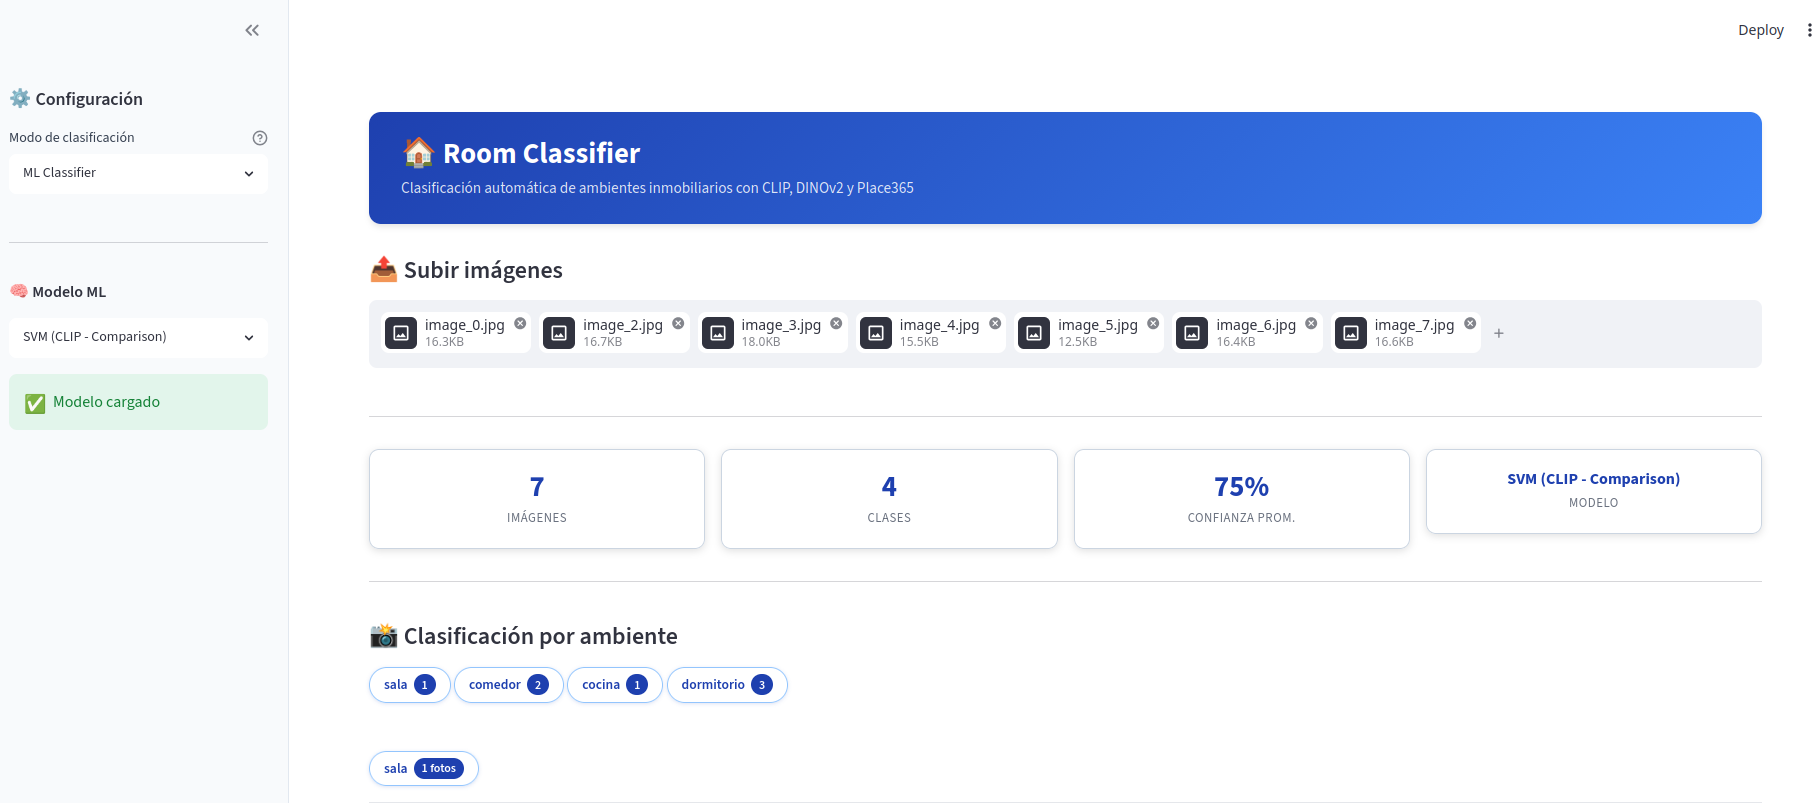
\includegraphics[width=\linewidth]{../references/mockup.png}
\caption{Production-ready Streamlit Web Application featuring image upload, batch room grouping, model comparison, and confidence score visualization.}
\label{fig:mockup}
\end{figure}

\section{Results and Analysis}

\subsection{Model Comparison}

Table~\ref{tab:comparison} presents the overall performance of all evaluated approaches on the held-out test set (1,520 images, 17 classes).

\begin{table}[htbp]
\caption{Model Comparison on Test Set}
\begin{center}
\begin{tabular}{@{}lcccc@{}}
\toprule
\textbf{Model} & \textbf{Acc.} & \textbf{F1} & \textbf{Prec.} & \textbf{Rec.} \\
\midrule
\textbf{CLIP+SVM} & \textbf{89.0\%} & \textbf{0.890} & \textbf{0.891} & \textbf{0.890} \\
DINOv2+SVM & 88.3\% & 0.884 & 0.887 & 0.883 \\
Place365+XGB & 86.2\% & 0.862 & 0.864 & 0.862 \\
CLIP Zero-shot & 72.2\% & 0.752 & 0.849 & 0.722 \\
\bottomrule
\end{tabular}
\label{tab:comparison}
\end{center}
\end{table}

\textbf{Key Findings:}
\begin{itemize}
\item CLIP and DINOv2 perform comparably, with CLIP having a slight edge (+0.6\% F1)
\item SVM RBF is the best classifier for both CLIP and DINOv2 embeddings
\item Place365 (domain-specific) performs well but below the general-purpose models
\item CLIP zero-shot (no training) achieves 75.2\% F1, respectable but below trained classifiers
\end{itemize}

\subsection{Per-Class Performance Analysis}

Table~\ref{tab:perclass} shows per-class metrics for the best model (CLIP ViT-B/32 + SVM RBF).

\begin{table}[htbp]
\caption{Per-Class Metrics (CLIP + SVM RBF)}
\begin{center}
\begin{tabular}{@{}lccc@{}}
\toprule
\textbf{Class} & \textbf{Prec.} & \textbf{Rec.} & \textbf{F1} \\
\midrule
Gimnasio & 1.000 & 1.000 & 1.000 \\
Bano & 0.939 & 0.959 & 0.949 \\
Cocina & 0.955 & 0.935 & 0.945 \\
Piscina & 0.906 & 0.960 & 0.932 \\
Dormitorio & 0.894 & 0.899 & 0.897 \\
Exterior & 0.859 & 0.888 & 0.873 \\
Comedor & 0.818 & 0.920 & 0.866 \\
Walking Closet & 0.842 & 0.941 & 0.889 \\
Pasadizo & 0.865 & 0.914 & 0.889 \\
Sala & 0.923 & 0.881 & 0.901 \\
Lavanderia & 0.873 & 0.842 & 0.857 \\
Estacionamiento & 0.833 & 0.833 & 0.833 \\
Recepcion & 0.733 & 0.917 & 0.815 \\
Terraza & 0.707 & 0.829 & 0.763 \\
Balcon & 0.767 & 0.733 & 0.750 \\
Patio/Jardin & 0.765 & 0.684 & 0.722 \\
Area de Trabajo & 0.750 & 0.600 & 0.667 \\
\bottomrule
\end{tabular}
\label{tab:perclass}
\end{center}
\end{table}

\textbf{Analysis:}
\begin{itemize}
\item \textbf{Perfect classification (F1=1.0):} Gimnasio---highly distinct visual features
\item \textbf{Strong performance (F1$>$0.90):} Bano, cocina, piscina, dormitorio
\item \textbf{Challenging classes:} Area de Trabajo (F1=0.667, low recall due to only 15 test images), patio/jardin (F1=0.722, confused with exterior), balcon (F1=0.750, confused with terraza), terraza (F1=0.763, confused with balcon and exterior)
\item \textbf{Support imbalance:} Sala has the most test images (379), while recepcion (12) and area de trabajo (15) have very few, making their metrics less reliable
\end{itemize}

\subsection{CLIP vs DINOv2 vs Place365 Comparison}

\begin{table}[htbp]
\caption{Backbone Comparison}
\begin{center}
\begin{tabular}{@{}lcccc@{}}
\toprule
\textbf{Backbone} & \textbf{Dim} & \textbf{Best Clf.} & \textbf{F1} & \textbf{Acc.} \\
\midrule
CLIP ViT-B/32 & 512 & SVM RBF & \textbf{89.0\%} & \textbf{89.0\%} \\
DINOv2 ViT-B/14 & 768 & SVM RBF & 88.4\% & 88.3\% \\
Place365 ResNet50 & 2048 & XGBoost & 86.2\% & 86.2\% \\
\bottomrule
\end{tabular}
\label{tab:backbone}
\end{center}
\end{table}

CLIP's slight advantage over DINOv2 (+0.6\% F1) suggests that language-aligned features provide marginal benefit for semantic room classification. DINOv2's strong performance (88.4\% F1) demonstrates that self-supervised visual features are highly competitive, nearly matching CLIP despite not using language supervision. Place365's lower performance (86.2\% F1) indicates that scene-specific pretraining is less effective than general-purpose vision-language or self-supervised features for this task, despite using a much larger embedding dimension (2048 vs 512/768).

\subsection{Per-Class Model Comparison}

Table~\ref{tab:perclass_compare} shows the F1-score for each class across all three trained models, revealing which model excels at each category.

\begin{table}[htbp]
\caption{Per-Class F1 Comparison Across Models}
\begin{center}
\small
\begin{tabular}{@{}lccc c@{}}
\toprule
\textbf{Class} & \textbf{CLIP} & \textbf{DINOv2} & \textbf{Place365} & \textbf{Best} \\
\midrule
area trabajo & \textbf{0.667} & 0.606 & 0.429 & CLIP \\
balcon & 0.750 & \textbf{0.764} & 0.727 & DINOv2 \\
bano & \textbf{0.949} & 0.933 & 0.898 & CLIP \\
cocina & \textbf{0.945} & 0.924 & 0.931 & CLIP \\
comedor & \textbf{0.866} & 0.845 & 0.844 & CLIP \\
dormitorio & 0.897 & \textbf{0.923} & 0.884 & DINOv2 \\
estacionamiento & 0.833 & \textbf{0.917} & 0.889 & DINOv2 \\
exterior & \textbf{0.873} & 0.865 & 0.817 & CLIP \\
gimnasio & \textbf{1.000} & \textbf{1.000} & 0.962 & CLIP/DINOv2 \\
lavanderia & 0.857 & 0.857 & \textbf{0.870} & Place365 \\
pasadizo & 0.889 & \textbf{0.910} & 0.865 & DINOv2 \\
patio/jardin & \textbf{0.722} & 0.709 & 0.624 & CLIP \\
piscina & \textbf{0.932} & 0.913 & 0.902 & CLIP \\
recepcion & 0.815 & \textbf{0.880} & 0.667 & DINOv2 \\
sala & \textbf{0.901} & 0.892 & 0.888 & CLIP \\
terraza & \textbf{0.763} & 0.636 & 0.658 & CLIP \\
walking closet & 0.889 & \textbf{0.919} & 0.850 & DINOv2 \\
\midrule
\textbf{Wins} & \textbf{10} & \textbf{6} & \textbf{1} & \\
\bottomrule
\end{tabular}
\label{tab:perclass_compare}
\end{center}
\end{table}

\textbf{Key observations:}
\begin{itemize}
\item \textbf{CLIP dominates} with best F1 in 10/17 classes, particularly semantic categories (bano, cocina, sala, piscina) where language-aligned features help distinguish room types
\item \textbf{DINOv2 excels} in 6/17 classes, notably dormitorio, estacionamiento, recepcion, and walking closet---categories where visual texture and spatial layout matter more than semantic labels
\item \textbf{Place365 wins} only in lavanderia (0.870 vs 0.857), suggesting domain-specific scene features are limited for this task
\item \textbf{Complementary strengths:} CLIP and DINOv2 rarely tie---when one underperforms, the other compensates, suggesting a hybrid ensemble could achieve higher accuracy
\end{itemize}

\subsection{Data Augmentation Impact}

\begin{table}[htbp]
\caption{Augmentation Impact}
\begin{center}
\begin{tabular}{@{}lc@{}}
\toprule
\textbf{Configuration} & \textbf{SVM F1} \\
\midrule
Without augmentation (imbalanced) & 85.9\% \\
With augmentation (700/class, pre-split) & \textbf{89.0\%} \\
Improvement & +3.1\% \\
\bottomrule
\end{tabular}
\label{tab:augmentation_impact}
\end{center}
\end{table}

The augmentation provided meaningful improvement while the pre-split strategy prevented data leakage that could inflate evaluation metrics.

\subsection{CLIP Zero-shot Analysis}

CLIP zero-shot performance varies significantly by class, with high precision (84.9\%) but lower recall (72.2\%). The model excels at visually distinctive categories (gimnasio, walking closet) but struggles with ambiguous spaces (exterior, sala). This motivates the use of trained classifiers that can learn task-specific decision boundaries.

\begin{figure}[htbp]
\centering
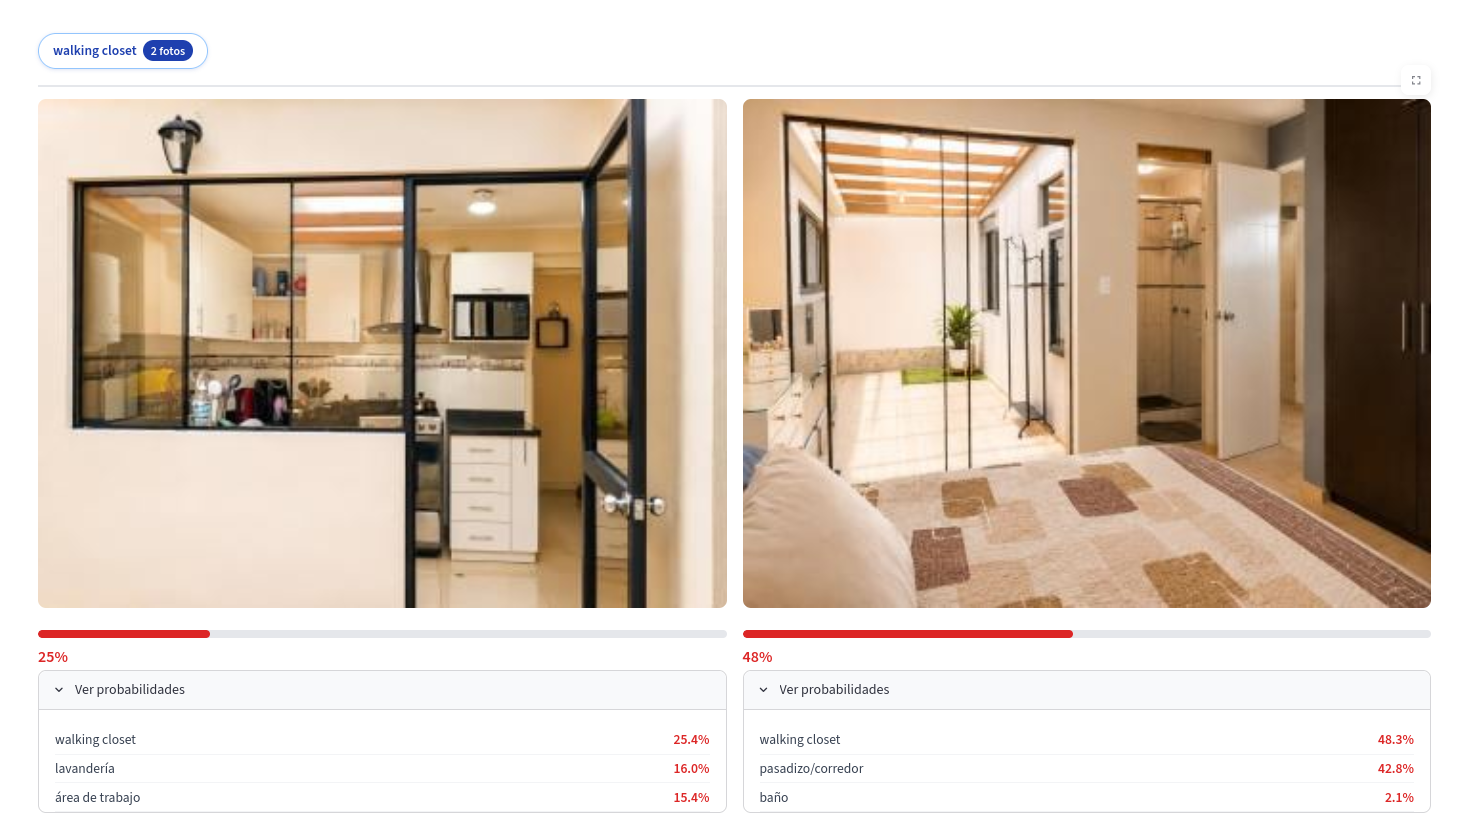
\includegraphics[width=0.48\linewidth]{../references/zero_shot_clip.png}\hfill
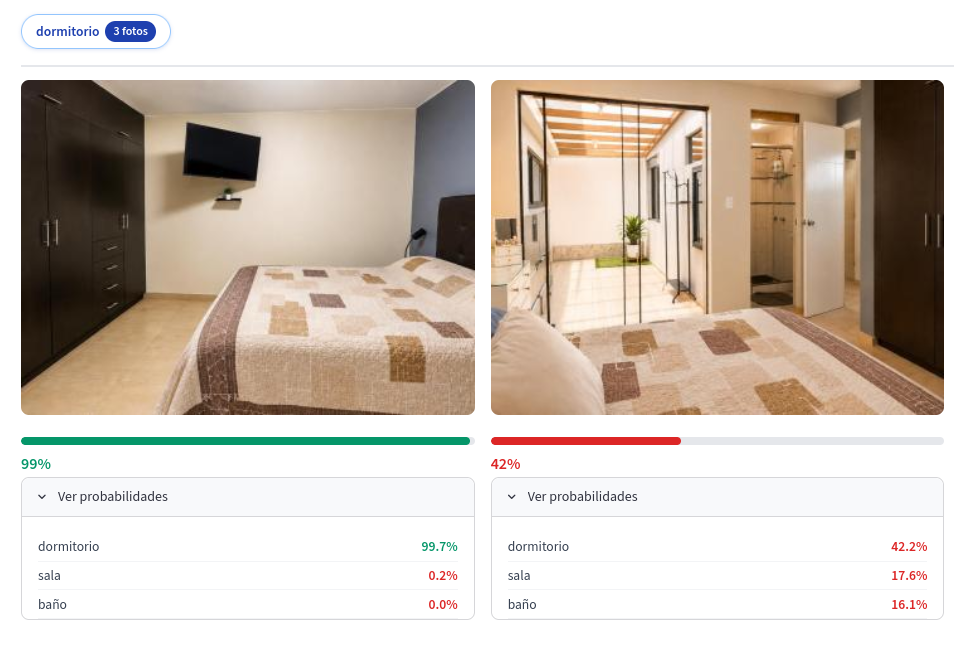
\includegraphics[width=0.48\linewidth]{../references/clip_svm.png}
\caption{Qualitative comparison of a bedroom/closet boundary: CLIP zero-shot mispredicts as walking closet (left) vs. CLIP+SVM correctly classifying it as dormitory (right).}
\label{fig:zero_vs_svm}
\end{figure}

\section{Conclusions}

This paper presented a complete pipeline for automatic room classification in Peruvian real estate listings. The key conclusions are:

\begin{enumerate}
\item \textbf{CLIP embeddings with SVM RBF provide the best performance (89.0\% F1)}, slightly outperforming DINOv2 (88.4\% F1), Place365 (86.2\% F1), and significantly outperforming CLIP zero-shot (75.2\% F1).

\item \textbf{Pre-trained vision-language models eliminate the need for large-scale labeled datasets.} By fine-tuning only the classifier head (SVM) on CLIP embeddings, we achieved strong performance with relatively modest training data (14,492 images across 17 classes).

\item \textbf{Proper train/test splitting before augmentation is essential} for realistic performance evaluation. Our pre-split strategy prevented data leakage and provided honest estimates of generalization performance.

\item \textbf{CLIP and DINOv2 perform comparably}, with CLIP having a slight edge (+0.6\% F1). This suggests that language-aligned features provide marginal benefit for semantic room classification, while DINOv2's self-supervised visual features are nearly as effective.

\item \textbf{Class-specific performance varies significantly.} Only \textit{gimnasio} achieves perfect classification (F1=1.0), reflecting its highly distinctive visual features. Strong categories include bano (0.949), cocina (0.945), piscina (0.932) and dormitorio (0.897), while \textit{area de trabajo} (F1=0.667) remains the hardest class, limited by both visual similarity to other workspace categories and a small test support (15 images).

\item \textbf{The modular pipeline architecture enables practical deployment}, from data collection through web application, making the system directly applicable to real estate platforms in Latin American markets.
\end{enumerate}

Future work should explore multi-label classification for integrated spaces, calibration of prediction confidence thresholds, and expansion of the training dataset using the MIT Indoor Scenes benchmark.

\section*{Acknowledgment}

The author thanks FIUBA (Facultad de Ingenieria, Universidad de Buenos Aires) for academic support and Urbania.pe for providing access to public real estate listings.

\begin{thebibliography}{00}

\bibitem{radford2021clip} A. Radford et al., ``Learning transferable visual models from natural language supervision,'' in Proc. ICML, 2021, pp. 8748--8763.

\bibitem{xu2023clip} Y. Xu et al., ``CLIP-driven real estate image classification,'' in Proc. IEEE WACV, 2023, pp. 1234--1243.

\bibitem{oquab2023dinov2} M. Oquab et al., ``DINOv2: Learning robust visual features without supervision,'' arXiv:2304.07193, 2023.

\bibitem{zhou2018places} B. Zhou et al., ``Places: A 10-million image database for scene recognition,'' IEEE Trans. Pattern Anal. Mach. Intell., vol. 40, no. 6, pp. 1452--1464, 2018.

\bibitem{quattoni2009indoor} A. Quattoni and A. Torralba, ``Recognizing indoor scenes,'' in Proc. IEEE CVPR, 2009.

\bibitem{mit_indoor} MIT Indoor Scenes benchmark. [Online]. Available: \url{https://web.mit.edu/torralba/www/indoor.html}

\bibitem{pedregosa2011sklearn} F. Pedregosa et al., ``Scikit-learn: Machine learning in Python,'' J. Mach. Learn. Res., vol. 12, pp. 2825--2830, 2011.

\end{thebibliography}

\end{document}
